\documentclass[twoside]{book}

% Packages required by doxygen
\usepackage{fixltx2e}
\usepackage{calc}
\usepackage{doxygen}
\usepackage{graphicx}
\usepackage[utf8]{inputenc}
\usepackage{makeidx}
\usepackage{multicol}
\usepackage{multirow}
\PassOptionsToPackage{warn}{textcomp}
\usepackage{textcomp}
\usepackage[nointegrals]{wasysym}
\usepackage[table]{xcolor}

% Font selection
\usepackage[T1]{fontenc}
\usepackage{mathptmx}
\usepackage[scaled=.90]{helvet}
\usepackage{courier}
\usepackage{amssymb}
\usepackage{sectsty}
\renewcommand{\familydefault}{\sfdefault}
\allsectionsfont{%
  \fontseries{bc}\selectfont%
  \color{darkgray}%
}
\renewcommand{\DoxyLabelFont}{%
  \fontseries{bc}\selectfont%
  \color{darkgray}%
}
\newcommand{\+}{\discretionary{\mbox{\scriptsize$\hookleftarrow$}}{}{}}

% Page & text layout
\usepackage{geometry}
\geometry{%
  a4paper,%
  top=2.5cm,%
  bottom=2.5cm,%
  left=2.5cm,%
  right=2.5cm%
}
\tolerance=750
\hfuzz=15pt
\hbadness=750
\setlength{\emergencystretch}{15pt}
\setlength{\parindent}{0cm}
\setlength{\parskip}{0.2cm}
\makeatletter
\renewcommand{\paragraph}{%
  \@startsection{paragraph}{4}{0ex}{-1.0ex}{1.0ex}{%
    \normalfont\normalsize\bfseries\SS@parafont%
  }%
}
\renewcommand{\subparagraph}{%
  \@startsection{subparagraph}{5}{0ex}{-1.0ex}{1.0ex}{%
    \normalfont\normalsize\bfseries\SS@subparafont%
  }%
}
\makeatother

% Headers & footers
\usepackage{fancyhdr}
\pagestyle{fancyplain}
\fancyhead[LE]{\fancyplain{}{\bfseries\thepage}}
\fancyhead[CE]{\fancyplain{}{}}
\fancyhead[RE]{\fancyplain{}{\bfseries\leftmark}}
\fancyhead[LO]{\fancyplain{}{\bfseries\rightmark}}
\fancyhead[CO]{\fancyplain{}{}}
\fancyhead[RO]{\fancyplain{}{\bfseries\thepage}}
\fancyfoot[LE]{\fancyplain{}{}}
\fancyfoot[CE]{\fancyplain{}{}}
\fancyfoot[RE]{\fancyplain{}{\bfseries\scriptsize Generated on Tue Oct 21 2014 13\+:52\+:41 for F\+W\+Framework by Doxygen }}
\fancyfoot[LO]{\fancyplain{}{\bfseries\scriptsize Generated on Tue Oct 21 2014 13\+:52\+:41 for F\+W\+Framework by Doxygen }}
\fancyfoot[CO]{\fancyplain{}{}}
\fancyfoot[RO]{\fancyplain{}{}}
\renewcommand{\footrulewidth}{0.4pt}
\renewcommand{\chaptermark}[1]{%
  \markboth{#1}{}%
}
\renewcommand{\sectionmark}[1]{%
  \markright{\thesection\ #1}%
}

% Indices & bibliography
\usepackage{natbib}
\usepackage[titles]{tocloft}
\setcounter{tocdepth}{3}
\setcounter{secnumdepth}{5}
\makeindex

% Hyperlinks (required, but should be loaded last)
\usepackage{ifpdf}
\ifpdf
  \usepackage[pdftex,pagebackref=true]{hyperref}
\else
  \usepackage[ps2pdf,pagebackref=true]{hyperref}
\fi
\hypersetup{%
  colorlinks=true,%
  linkcolor=blue,%
  citecolor=blue,%
  unicode%
}

% Custom commands
\newcommand{\clearemptydoublepage}{%
  \newpage{\pagestyle{empty}\cleardoublepage}%
}


%===== C O N T E N T S =====

\begin{document}

% Titlepage & ToC
\hypersetup{pageanchor=false,
             bookmarks=true,
             bookmarksnumbered=true,
             pdfencoding=unicode
            }
\pagenumbering{roman}
\begin{titlepage}
\vspace*{7cm}
\begin{center}%
{\Large F\+W\+Framework \\[1ex]\large 1.\+0 }\\
\vspace*{1cm}
{\large Generated by Doxygen 1.8.8}\\
\vspace*{0.5cm}
{\small Tue Oct 21 2014 13:52:41}\\
\end{center}
\end{titlepage}
\clearemptydoublepage
\tableofcontents
\clearemptydoublepage
\pagenumbering{arabic}
\hypersetup{pageanchor=true}

%--- Begin generated contents ---
\chapter{Hierarchical Index}
\section{Class Hierarchy}
This inheritance list is sorted roughly, but not completely, alphabetically\+:\begin{DoxyCompactList}
\item \contentsline{section}{Color}{\pageref{struct_color}}{}
\item \contentsline{section}{F\+W\+Application}{\pageref{class_f_w_application}}{}
\item \contentsline{section}{I\+Game\+Object}{\pageref{class_i_game_object}}{}
\begin{DoxyCompactList}
\item \contentsline{section}{Monster}{\pageref{class_monster}}{}
\end{DoxyCompactList}
\end{DoxyCompactList}

\chapter{Class Index}
\section{Class List}
Here are the classes, structs, unions and interfaces with brief descriptions\+:\begin{DoxyCompactList}
\item\contentsline{section}{\hyperlink{struct_color}{Color} }{\pageref{struct_color}}{}
\item\contentsline{section}{\hyperlink{class_f_w_application}{F\+W\+Application} }{\pageref{class_f_w_application}}{}
\item\contentsline{section}{\hyperlink{class_i_game_object}{I\+Game\+Object} }{\pageref{class_i_game_object}}{}
\item\contentsline{section}{\hyperlink{class_monster}{Monster} }{\pageref{class_monster}}{}
\end{DoxyCompactList}

\chapter{Class Documentation}
\hypertarget{struct_color}{\section{Color Struct Reference}
\label{struct_color}\index{Color@{Color}}
}
\subsection*{Public Member Functions}
\begin{DoxyCompactItemize}
\item 
\hypertarget{struct_color_ae47bf1bef1dfe52a8300239e46b50122}{{\bfseries Color} (uint32\+\_\+t red, uint32\+\_\+t green, uint32\+\_\+t blue, uint32\+\_\+t alpha)}\label{struct_color_ae47bf1bef1dfe52a8300239e46b50122}

\end{DoxyCompactItemize}
\subsection*{Public Attributes}
\begin{DoxyCompactItemize}
\item 
\hypertarget{struct_color_a3249a9e784a2f087bde25f9c3cf2700d}{uint32\+\_\+t {\bfseries r}}\label{struct_color_a3249a9e784a2f087bde25f9c3cf2700d}

\item 
\hypertarget{struct_color_a6b92bc7134b6e016d2a04813cad97638}{uint32\+\_\+t {\bfseries g}}\label{struct_color_a6b92bc7134b6e016d2a04813cad97638}

\item 
\hypertarget{struct_color_a24ff460ba4d95b3ff221757e6fd8246e}{uint32\+\_\+t {\bfseries b}}\label{struct_color_a24ff460ba4d95b3ff221757e6fd8246e}

\item 
\hypertarget{struct_color_a5522bf0c5397a8e0e05b0cccc291b510}{uint32\+\_\+t {\bfseries a}}\label{struct_color_a5522bf0c5397a8e0e05b0cccc291b510}

\end{DoxyCompactItemize}


The documentation for this struct was generated from the following file\+:\begin{DoxyCompactItemize}
\item 
F\+W\+Application.\+h\end{DoxyCompactItemize}

\hypertarget{class_f_w_application}{\section{F\+W\+Application Class Reference}
\label{class_f_w_application}\index{F\+W\+Application@{F\+W\+Application}}
}
\subsection*{Public Member Functions}
\begin{DoxyCompactItemize}
\item 
\hypertarget{class_f_w_application_a9d9ae1cd8e16ecb6c31990c39629067f}{{\bfseries F\+W\+Application} (int offset\+X=50, int offset\+Y=50, int width=800, int height=600)}\label{class_f_w_application_a9d9ae1cd8e16ecb6c31990c39629067f}

\item 
\hypertarget{class_f_w_application_a109e3927f7da9c5301fd5512f64178f2}{void {\bfseries Set\+Target\+F\+P\+S} (unsigned short target)}\label{class_f_w_application_a109e3927f7da9c5301fd5512f64178f2}

\item 
S\+D\+L\+\_\+\+Window $\ast$ \hyperlink{class_f_w_application_a0bd2e7dab8d26d674ec89803ab4789d3}{Get\+Window} () const 
\begin{DoxyCompactList}\small\item\em Gets the window. \end{DoxyCompactList}\item 
bool \hyperlink{class_f_w_application_ae8002752e6cf2a9a602a55a0f8db2873}{Is\+Running} ()
\begin{DoxyCompactList}\small\item\em Is the game running, returns false when window is closed. \end{DoxyCompactList}\item 
std\+::string \hyperlink{class_f_w_application_a3d6a38a6314d281f6793d24951eaaed7}{Get\+Relative\+Path} (const std\+::string \&path=\char`\"{}\char`\"{}) const 
\begin{DoxyCompactList}\small\item\em Returns a relative path at the binary location \end{DoxyCompactList}\item 
S\+D\+L\+\_\+\+Texture $\ast$ \hyperlink{class_f_w_application_aa103aa5ee7cdbe5e2cae01fcdfb19472}{Load\+Texture} (const std\+::string \&file\+Name)
\begin{DoxyCompactList}\small\item\em Loads a texture and returns it's pointer. Note you have to cleanup yourself \end{DoxyCompactList}\item 
void \hyperlink{class_f_w_application_a015406b6f70c8edb674bb0f50516500c}{Draw\+Texture} (S\+D\+L\+\_\+\+Texture $\ast$texture, int x\+Offset, int y\+Offset)
\begin{DoxyCompactList}\small\item\em Draw a texture to the screen at a given position \end{DoxyCompactList}\item 
void \hyperlink{class_f_w_application_a6d9a4dc3068d15272c143b89cc22934e}{Draw\+Texture} (S\+D\+L\+\_\+\+Texture $\ast$texture, int x\+Offset, int y\+Offset, int width, int height)
\begin{DoxyCompactList}\small\item\em Draw a texture to the screen at a given position \end{DoxyCompactList}\item 
void \hyperlink{class_f_w_application_aace2f8e1125300546dc796cf74e34314}{Draw\+Line} (int start\+Pos\+X, int start\+Pos\+Y, int end\+Pos\+X, int end\+Pos\+Y)
\begin{DoxyCompactList}\small\item\em Draws a line from position to position \end{DoxyCompactList}\item 
void \hyperlink{class_f_w_application_a5e8cd6326546fba991c787a481b7005c}{Draw\+Rect} (int start\+Pos\+X, int start\+Pos\+Y, int width, int height, bool fill)
\begin{DoxyCompactList}\small\item\em Draws a rect from start position to end position \end{DoxyCompactList}\item 
void \hyperlink{class_f_w_application_a9af3769859c50a445ef8f0a08fc548ae}{Draw\+Text} (const std\+::string \&message, uint32\+\_\+t offset\+X, uint32\+\_\+t offset\+Y)
\begin{DoxyCompactList}\small\item\em Draws text on the screen at a given location \end{DoxyCompactList}\item 
void \hyperlink{class_f_w_application_a7b04b6b13c221cf67728a7d6372c838c}{Start\+Tick} ()
\begin{DoxyCompactList}\small\item\em Start of the cycle, catches input, etc. \end{DoxyCompactList}\item 
void \hyperlink{class_f_w_application_a6c5dbaaef4d13b0cf17727f8f84ef0fc}{End\+Tick} ()
\begin{DoxyCompactList}\small\item\em End of the cycle, swaps buffers \end{DoxyCompactList}\item 
void \hyperlink{class_f_w_application_afd869f6c0bf21b8bdc780ca9d513553f}{Remove\+Texture} (S\+D\+L\+\_\+\+Texture $\ast$texture)
\begin{DoxyCompactList}\small\item\em Destroy a texture resource, and frees memory \end{DoxyCompactList}\item 
void \hyperlink{class_f_w_application_a45ce0cbf998ae9ed2c79c7bd73f8782a}{Set\+Color} (const \hyperlink{struct_color}{Color} \&color)
\begin{DoxyCompactList}\small\item\em Set the color (as a state), all future draws are done with this color. \end{DoxyCompactList}\item 
void \hyperlink{class_f_w_application_a014258fb16a8eb170f38469bfb369166}{Set\+Font} (const std\+::string \&file\+Name)
\begin{DoxyCompactList}\small\item\em Sets the font as a state, all future font rendering is done with this font. \end{DoxyCompactList}\item 
void \hyperlink{class_f_w_application_ae59b00bb00d57974a74846af02fc58db}{Set\+Font\+Size} (int pt\+Size)
\begin{DoxyCompactList}\small\item\em Sets the fontsize as a state, all future font rendering is done in this size. \end{DoxyCompactList}\item 
void \hyperlink{class_f_w_application_a97b8073420aec9a721408bde5d31ee9f}{Add\+Renderable} (\hyperlink{class_i_game_object}{I\+Game\+Object} $\ast$renderable)
\begin{DoxyCompactList}\small\item\em Add a renderable object, update and render will be called when ticks are handled by the application. \end{DoxyCompactList}\item 
\hypertarget{class_f_w_application_a40ce413be238be95a8815b0d0a474d75}{uint32\+\_\+t {\bfseries Get\+Time\+Since\+Started\+M\+S} () const }\label{class_f_w_application_a40ce413be238be95a8815b0d0a474d75}

\item 
void \hyperlink{class_f_w_application_a57e09a281fc706a0622f7204aaeb6bbe}{Update\+Game\+Objects} ()
\begin{DoxyCompactList}\small\item\em Updates all game\+Objects \end{DoxyCompactList}\item 
void \hyperlink{class_f_w_application_a1a9208982cc76086430616eaf7e88568}{Render\+Game\+Objects} ()
\begin{DoxyCompactList}\small\item\em Renders all game\+Objects \end{DoxyCompactList}\end{DoxyCompactItemize}
\subsection*{Static Public Member Functions}
\begin{DoxyCompactItemize}
\item 
\hypertarget{class_f_w_application_ad52cf42e501e932275bca974ca32f4f7}{static \hyperlink{class_f_w_application}{F\+W\+Application} $\ast$ {\bfseries Get\+Instance} ()}\label{class_f_w_application_ad52cf42e501e932275bca974ca32f4f7}

\end{DoxyCompactItemize}


\subsection{Member Function Documentation}
\hypertarget{class_f_w_application_a97b8073420aec9a721408bde5d31ee9f}{\index{F\+W\+Application@{F\+W\+Application}!Add\+Renderable@{Add\+Renderable}}
\index{Add\+Renderable@{Add\+Renderable}!F\+W\+Application@{F\+W\+Application}}
\subsubsection[{Add\+Renderable}]{\setlength{\rightskip}{0pt plus 5cm}void F\+W\+Application\+::\+Add\+Renderable (
\begin{DoxyParamCaption}
\item[{{\bf I\+Game\+Object} $\ast$}]{renderable}
\end{DoxyParamCaption}
)}}\label{class_f_w_application_a97b8073420aec9a721408bde5d31ee9f}


Add a renderable object, update and render will be called when ticks are handled by the application. 

Joris, 21-\/10-\/2014. 


\begin{DoxyParams}{Parameters}
{\em renderable} & \mbox{[}in,out\mbox{]} If non-\/null, the renderable. \\
\hline
\end{DoxyParams}
\hypertarget{class_f_w_application_aace2f8e1125300546dc796cf74e34314}{\index{F\+W\+Application@{F\+W\+Application}!Draw\+Line@{Draw\+Line}}
\index{Draw\+Line@{Draw\+Line}!F\+W\+Application@{F\+W\+Application}}
\subsubsection[{Draw\+Line}]{\setlength{\rightskip}{0pt plus 5cm}void F\+W\+Application\+::\+Draw\+Line (
\begin{DoxyParamCaption}
\item[{int}]{start\+Pos\+X, }
\item[{int}]{start\+Pos\+Y, }
\item[{int}]{end\+Pos\+X, }
\item[{int}]{end\+Pos\+Y}
\end{DoxyParamCaption}
)}}\label{class_f_w_application_aace2f8e1125300546dc796cf74e34314}


Draws a line from position to position 

Joris, 21-\/10-\/2014. 


\begin{DoxyParams}{Parameters}
{\em start\+Pos\+X} & The start position x coordinate. \\
\hline
{\em start\+Pos\+Y} & The start position y coordinate. \\
\hline
{\em end\+Pos\+X} & The end position x coordinate. \\
\hline
{\em end\+Pos\+Y} & The end position y coordinate. \\
\hline
\end{DoxyParams}
\hypertarget{class_f_w_application_a5e8cd6326546fba991c787a481b7005c}{\index{F\+W\+Application@{F\+W\+Application}!Draw\+Rect@{Draw\+Rect}}
\index{Draw\+Rect@{Draw\+Rect}!F\+W\+Application@{F\+W\+Application}}
\subsubsection[{Draw\+Rect}]{\setlength{\rightskip}{0pt plus 5cm}void F\+W\+Application\+::\+Draw\+Rect (
\begin{DoxyParamCaption}
\item[{int}]{start\+Pos\+X, }
\item[{int}]{start\+Pos\+Y, }
\item[{int}]{width, }
\item[{int}]{height, }
\item[{bool}]{fill}
\end{DoxyParamCaption}
)}}\label{class_f_w_application_a5e8cd6326546fba991c787a481b7005c}


Draws a rect from start position to end position 

Joris, 21-\/10-\/2014. 


\begin{DoxyParams}{Parameters}
{\em start\+Pos\+X} & The start position x coordinate. \\
\hline
{\em start\+Pos\+Y} & The start position y coordinate. \\
\hline
{\em width} & The width. \\
\hline
{\em height} & The height. \\
\hline
{\em fill} & true to fill. \\
\hline
\end{DoxyParams}
\hypertarget{class_f_w_application_a9af3769859c50a445ef8f0a08fc548ae}{\index{F\+W\+Application@{F\+W\+Application}!Draw\+Text@{Draw\+Text}}
\index{Draw\+Text@{Draw\+Text}!F\+W\+Application@{F\+W\+Application}}
\subsubsection[{Draw\+Text}]{\setlength{\rightskip}{0pt plus 5cm}void F\+W\+Application\+::\+Draw\+Text (
\begin{DoxyParamCaption}
\item[{const std\+::string \&}]{message, }
\item[{uint32\+\_\+t}]{offset\+X, }
\item[{uint32\+\_\+t}]{offset\+Y}
\end{DoxyParamCaption}
)}}\label{class_f_w_application_a9af3769859c50a445ef8f0a08fc548ae}


Draws text on the screen at a given location 

Joris, 21-\/10-\/2014. 


\begin{DoxyParams}{Parameters}
{\em message} & The message. \\
\hline
{\em offset\+X} & The offset x coordinate. \\
\hline
{\em offset\+Y} & The offset y coordinate. \\
\hline
\end{DoxyParams}
\hypertarget{class_f_w_application_a015406b6f70c8edb674bb0f50516500c}{\index{F\+W\+Application@{F\+W\+Application}!Draw\+Texture@{Draw\+Texture}}
\index{Draw\+Texture@{Draw\+Texture}!F\+W\+Application@{F\+W\+Application}}
\subsubsection[{Draw\+Texture}]{\setlength{\rightskip}{0pt plus 5cm}void F\+W\+Application\+::\+Draw\+Texture (
\begin{DoxyParamCaption}
\item[{S\+D\+L\+\_\+\+Texture $\ast$}]{texture, }
\item[{int}]{x\+Offset, }
\item[{int}]{y\+Offset}
\end{DoxyParamCaption}
)}}\label{class_f_w_application_a015406b6f70c8edb674bb0f50516500c}


Draw a texture to the screen at a given position 

Joris, 21-\/10-\/2014. 


\begin{DoxyParams}{Parameters}
{\em texture} & \mbox{[}in,out\mbox{]} If non-\/null, the texture. \\
\hline
{\em x\+Offset} & The offset. \\
\hline
{\em y\+Offset} & The offset. \\
\hline
\end{DoxyParams}
\hypertarget{class_f_w_application_a6d9a4dc3068d15272c143b89cc22934e}{\index{F\+W\+Application@{F\+W\+Application}!Draw\+Texture@{Draw\+Texture}}
\index{Draw\+Texture@{Draw\+Texture}!F\+W\+Application@{F\+W\+Application}}
\subsubsection[{Draw\+Texture}]{\setlength{\rightskip}{0pt plus 5cm}void F\+W\+Application\+::\+Draw\+Texture (
\begin{DoxyParamCaption}
\item[{S\+D\+L\+\_\+\+Texture $\ast$}]{texture, }
\item[{int}]{x\+Offset, }
\item[{int}]{y\+Offset, }
\item[{int}]{width, }
\item[{int}]{height}
\end{DoxyParamCaption}
)}}\label{class_f_w_application_a6d9a4dc3068d15272c143b89cc22934e}


Draw a texture to the screen at a given position 

Joris, 21-\/10-\/2014. 


\begin{DoxyParams}{Parameters}
{\em texture} & \mbox{[}in,out\mbox{]} If non-\/null, the texture. \\
\hline
{\em x\+Offset} & The offset. \\
\hline
{\em y\+Offset} & The offset. \\
\hline
{\em width} & The width. \\
\hline
{\em height} & The height. \\
\hline
\end{DoxyParams}
\hypertarget{class_f_w_application_a6c5dbaaef4d13b0cf17727f8f84ef0fc}{\index{F\+W\+Application@{F\+W\+Application}!End\+Tick@{End\+Tick}}
\index{End\+Tick@{End\+Tick}!F\+W\+Application@{F\+W\+Application}}
\subsubsection[{End\+Tick}]{\setlength{\rightskip}{0pt plus 5cm}void F\+W\+Application\+::\+End\+Tick (
\begin{DoxyParamCaption}
{}
\end{DoxyParamCaption}
)}}\label{class_f_w_application_a6c5dbaaef4d13b0cf17727f8f84ef0fc}


End of the cycle, swaps buffers 

Joris, 21-\/10-\/2014. \hypertarget{class_f_w_application_a3d6a38a6314d281f6793d24951eaaed7}{\index{F\+W\+Application@{F\+W\+Application}!Get\+Relative\+Path@{Get\+Relative\+Path}}
\index{Get\+Relative\+Path@{Get\+Relative\+Path}!F\+W\+Application@{F\+W\+Application}}
\subsubsection[{Get\+Relative\+Path}]{\setlength{\rightskip}{0pt plus 5cm}std\+::string F\+W\+Application\+::\+Get\+Relative\+Path (
\begin{DoxyParamCaption}
\item[{const std\+::string \&}]{path = {\ttfamily \char`\"{}\char`\"{}}}
\end{DoxyParamCaption}
) const}}\label{class_f_w_application_a3d6a38a6314d281f6793d24951eaaed7}


Returns a relative path at the binary location 

Joris, 21-\/10-\/2014. 


\begin{DoxyParams}{Parameters}
{\em path} & (Optional) full pathname of the file. \\
\hline
\end{DoxyParams}


\begin{DoxyReturn}{Returns}
The relative path. 
\end{DoxyReturn}
\hypertarget{class_f_w_application_a0bd2e7dab8d26d674ec89803ab4789d3}{\index{F\+W\+Application@{F\+W\+Application}!Get\+Window@{Get\+Window}}
\index{Get\+Window@{Get\+Window}!F\+W\+Application@{F\+W\+Application}}
\subsubsection[{Get\+Window}]{\setlength{\rightskip}{0pt plus 5cm}S\+D\+L\+\_\+\+Window $\ast$ F\+W\+Application\+::\+Get\+Window (
\begin{DoxyParamCaption}
{}
\end{DoxyParamCaption}
) const}}\label{class_f_w_application_a0bd2e7dab8d26d674ec89803ab4789d3}


Gets the window. 

Joris, 21-\/10-\/2014. 

\begin{DoxyReturn}{Returns}
The S\+D\+L window. 
\end{DoxyReturn}
\hypertarget{class_f_w_application_ae8002752e6cf2a9a602a55a0f8db2873}{\index{F\+W\+Application@{F\+W\+Application}!Is\+Running@{Is\+Running}}
\index{Is\+Running@{Is\+Running}!F\+W\+Application@{F\+W\+Application}}
\subsubsection[{Is\+Running}]{\setlength{\rightskip}{0pt plus 5cm}bool F\+W\+Application\+::\+Is\+Running (
\begin{DoxyParamCaption}
{}
\end{DoxyParamCaption}
)}}\label{class_f_w_application_ae8002752e6cf2a9a602a55a0f8db2873}


Is the game running, returns false when window is closed. 

Joris, 21-\/10-\/2014. 

\begin{DoxyReturn}{Returns}
true if running, false if not. 
\end{DoxyReturn}
\hypertarget{class_f_w_application_aa103aa5ee7cdbe5e2cae01fcdfb19472}{\index{F\+W\+Application@{F\+W\+Application}!Load\+Texture@{Load\+Texture}}
\index{Load\+Texture@{Load\+Texture}!F\+W\+Application@{F\+W\+Application}}
\subsubsection[{Load\+Texture}]{\setlength{\rightskip}{0pt plus 5cm}S\+D\+L\+\_\+\+Texture $\ast$ F\+W\+Application\+::\+Load\+Texture (
\begin{DoxyParamCaption}
\item[{const std\+::string \&}]{file\+Name}
\end{DoxyParamCaption}
)}}\label{class_f_w_application_aa103aa5ee7cdbe5e2cae01fcdfb19472}


Loads a texture and returns it's pointer. Note you have to cleanup yourself 

Joris, 21-\/10-\/2014. 


\begin{DoxyParams}{Parameters}
{\em file\+Name} & Filename of the file. \\
\hline
\end{DoxyParams}


\begin{DoxyReturn}{Returns}
null if it fails, else the texture. 
\end{DoxyReturn}
\hypertarget{class_f_w_application_afd869f6c0bf21b8bdc780ca9d513553f}{\index{F\+W\+Application@{F\+W\+Application}!Remove\+Texture@{Remove\+Texture}}
\index{Remove\+Texture@{Remove\+Texture}!F\+W\+Application@{F\+W\+Application}}
\subsubsection[{Remove\+Texture}]{\setlength{\rightskip}{0pt plus 5cm}void F\+W\+Application\+::\+Remove\+Texture (
\begin{DoxyParamCaption}
\item[{S\+D\+L\+\_\+\+Texture $\ast$}]{texture}
\end{DoxyParamCaption}
)}}\label{class_f_w_application_afd869f6c0bf21b8bdc780ca9d513553f}


Destroy a texture resource, and frees memory 

Joris, 21-\/10-\/2014. 


\begin{DoxyParams}{Parameters}
{\em texture} & \mbox{[}in,out\mbox{]} If non-\/null, the texture. \\
\hline
\end{DoxyParams}
\hypertarget{class_f_w_application_a1a9208982cc76086430616eaf7e88568}{\index{F\+W\+Application@{F\+W\+Application}!Render\+Game\+Objects@{Render\+Game\+Objects}}
\index{Render\+Game\+Objects@{Render\+Game\+Objects}!F\+W\+Application@{F\+W\+Application}}
\subsubsection[{Render\+Game\+Objects}]{\setlength{\rightskip}{0pt plus 5cm}void F\+W\+Application\+::\+Render\+Game\+Objects (
\begin{DoxyParamCaption}
{}
\end{DoxyParamCaption}
)}}\label{class_f_w_application_a1a9208982cc76086430616eaf7e88568}


Renders all game\+Objects 

Joris, 21-\/10-\/2014. \hypertarget{class_f_w_application_a45ce0cbf998ae9ed2c79c7bd73f8782a}{\index{F\+W\+Application@{F\+W\+Application}!Set\+Color@{Set\+Color}}
\index{Set\+Color@{Set\+Color}!F\+W\+Application@{F\+W\+Application}}
\subsubsection[{Set\+Color}]{\setlength{\rightskip}{0pt plus 5cm}void F\+W\+Application\+::\+Set\+Color (
\begin{DoxyParamCaption}
\item[{const {\bf Color} \&}]{color}
\end{DoxyParamCaption}
)}}\label{class_f_w_application_a45ce0cbf998ae9ed2c79c7bd73f8782a}


Set the color (as a state), all future draws are done with this color. 

Joris, 21-\/10-\/2014. 


\begin{DoxyParams}{Parameters}
{\em color} & The color. \\
\hline
\end{DoxyParams}
\hypertarget{class_f_w_application_a014258fb16a8eb170f38469bfb369166}{\index{F\+W\+Application@{F\+W\+Application}!Set\+Font@{Set\+Font}}
\index{Set\+Font@{Set\+Font}!F\+W\+Application@{F\+W\+Application}}
\subsubsection[{Set\+Font}]{\setlength{\rightskip}{0pt plus 5cm}void F\+W\+Application\+::\+Set\+Font (
\begin{DoxyParamCaption}
\item[{const std\+::string \&}]{file\+Name}
\end{DoxyParamCaption}
)}}\label{class_f_w_application_a014258fb16a8eb170f38469bfb369166}


Sets the font as a state, all future font rendering is done with this font. 

Joris, 21-\/10-\/2014. 


\begin{DoxyParams}{Parameters}
{\em file\+Name} & Filename of the file. \\
\hline
\end{DoxyParams}
\hypertarget{class_f_w_application_ae59b00bb00d57974a74846af02fc58db}{\index{F\+W\+Application@{F\+W\+Application}!Set\+Font\+Size@{Set\+Font\+Size}}
\index{Set\+Font\+Size@{Set\+Font\+Size}!F\+W\+Application@{F\+W\+Application}}
\subsubsection[{Set\+Font\+Size}]{\setlength{\rightskip}{0pt plus 5cm}void F\+W\+Application\+::\+Set\+Font\+Size (
\begin{DoxyParamCaption}
\item[{int}]{pt\+Size}
\end{DoxyParamCaption}
)}}\label{class_f_w_application_ae59b00bb00d57974a74846af02fc58db}


Sets the fontsize as a state, all future font rendering is done in this size. 

Joris, 21-\/10-\/2014. 


\begin{DoxyParams}{Parameters}
{\em pt\+Size} & Size of the point. \\
\hline
\end{DoxyParams}
\hypertarget{class_f_w_application_a7b04b6b13c221cf67728a7d6372c838c}{\index{F\+W\+Application@{F\+W\+Application}!Start\+Tick@{Start\+Tick}}
\index{Start\+Tick@{Start\+Tick}!F\+W\+Application@{F\+W\+Application}}
\subsubsection[{Start\+Tick}]{\setlength{\rightskip}{0pt plus 5cm}void F\+W\+Application\+::\+Start\+Tick (
\begin{DoxyParamCaption}
{}
\end{DoxyParamCaption}
)}}\label{class_f_w_application_a7b04b6b13c221cf67728a7d6372c838c}


Start of the cycle, catches input, etc. 

Joris, 21-\/10-\/2014. \hypertarget{class_f_w_application_a57e09a281fc706a0622f7204aaeb6bbe}{\index{F\+W\+Application@{F\+W\+Application}!Update\+Game\+Objects@{Update\+Game\+Objects}}
\index{Update\+Game\+Objects@{Update\+Game\+Objects}!F\+W\+Application@{F\+W\+Application}}
\subsubsection[{Update\+Game\+Objects}]{\setlength{\rightskip}{0pt plus 5cm}void F\+W\+Application\+::\+Update\+Game\+Objects (
\begin{DoxyParamCaption}
{}
\end{DoxyParamCaption}
)}}\label{class_f_w_application_a57e09a281fc706a0622f7204aaeb6bbe}


Updates all game\+Objects 

Joris, 21-\/10-\/2014. 

The documentation for this class was generated from the following files\+:\begin{DoxyCompactItemize}
\item 
F\+W\+Application.\+h\item 
F\+W\+Application.\+cpp\end{DoxyCompactItemize}

\hypertarget{class_i_game_object}{\section{I\+Game\+Object Class Reference}
\label{class_i_game_object}\index{I\+Game\+Object@{I\+Game\+Object}}
}
Inheritance diagram for I\+Game\+Object\+:\begin{figure}[H]
\begin{center}
\leavevmode
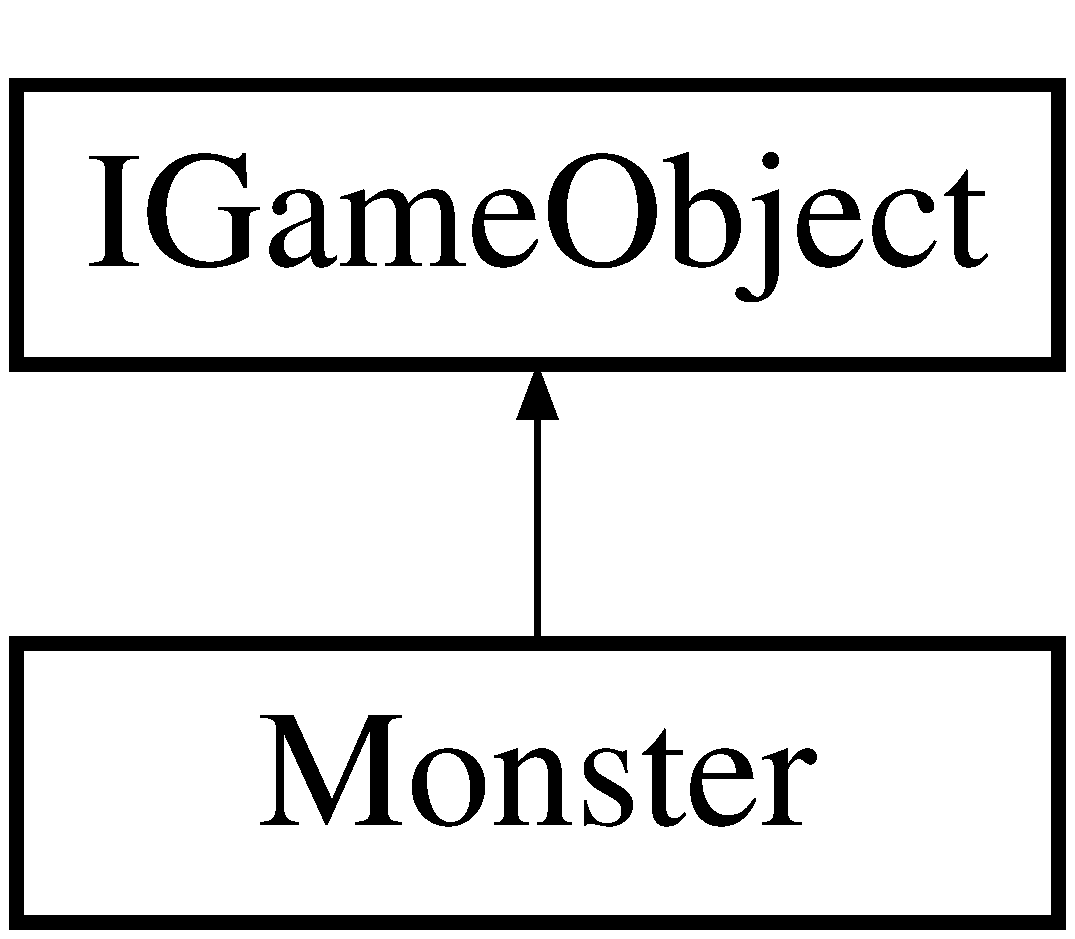
\includegraphics[height=2.000000cm]{class_i_game_object}
\end{center}
\end{figure}
\subsection*{Public Member Functions}
\begin{DoxyCompactItemize}
\item 
virtual void \hyperlink{class_i_game_object_aabf746343989a0a29543a3d6db48b6a4}{Draw} ()=0
\begin{DoxyCompactList}\small\item\em Abstract draw method \end{DoxyCompactList}\item 
virtual void \hyperlink{class_i_game_object_a4959cd2f80334cfa1a97255082e984cc}{Update} (float delta\+Time)=0
\begin{DoxyCompactList}\small\item\em Abstract update method \end{DoxyCompactList}\item 
virtual void \hyperlink{class_i_game_object_a31702eed0f78cff5e5d49717751bd39d}{On\+Collision} (\hyperlink{class_i_game_object}{I\+Game\+Object} $\ast$collided\+Object)=0
\begin{DoxyCompactList}\small\item\em Abstract on\+Collision method \end{DoxyCompactList}\item 
virtual void \hyperlink{class_i_game_object_abef2c39177245bdca445db64a1d24be8}{Set\+Offset} (uint32\+\_\+t x, uint32\+\_\+t y)
\begin{DoxyCompactList}\small\item\em Set the offset of this object (translation) \end{DoxyCompactList}\item 
virtual void \hyperlink{class_i_game_object_a133dd7afcf061416f25135e2d29412f9}{Get\+Offset} (uint32\+\_\+t \&x, uint32\+\_\+t \&y) const 
\begin{DoxyCompactList}\small\item\em Get the offset of this object (translation) \end{DoxyCompactList}\item 
virtual void \hyperlink{class_i_game_object_a1eddecf9e89fc2df118e2a801bf01875}{Set\+Size} (uint32\+\_\+t width, uint32\+\_\+t height)
\begin{DoxyCompactList}\small\item\em Set the bounding box of this object. \end{DoxyCompactList}\item 
virtual void \hyperlink{class_i_game_object_ace84e8ce58a6886028f2ada293a170c7}{Get\+Size} (uint32\+\_\+t \&width, uint32\+\_\+t \&height) const 
\begin{DoxyCompactList}\small\item\em Get the bounding box of this object. \end{DoxyCompactList}\item 
virtual void \hyperlink{class_i_game_object_a0c27f50dd3783bdc126beb249dc160d0}{Translate} (uint32\+\_\+t x, uint32\+\_\+t y)
\begin{DoxyCompactList}\small\item\em Move this object by a given amount. \end{DoxyCompactList}\item 
virtual void \hyperlink{class_i_game_object_a6c4babfa9e8eadd50599e5b7c4dd9e12}{Set\+Texture} (S\+D\+L\+\_\+\+Texture $\ast$texture)
\begin{DoxyCompactList}\small\item\em Set the texture of this object. \end{DoxyCompactList}\item 
virtual S\+D\+L\+\_\+\+Texture $\ast$ \hyperlink{class_i_game_object_af2a85a8821cbe4305ce92c8bbe8ecf5e}{Get\+Texture} () const 
\begin{DoxyCompactList}\small\item\em Get the texture of this object. \end{DoxyCompactList}\item 
virtual float \hyperlink{class_i_game_object_a0ef5e610a6afc8215902853820a7e954}{Distance\+To} (\hyperlink{class_i_game_object}{I\+Game\+Object} $\ast$obj)
\begin{DoxyCompactList}\small\item\em Get the distance to another object \end{DoxyCompactList}\item 
virtual float \hyperlink{class_i_game_object_ad34f7ba9433ba5e449852593011ffb6a}{Distance\+To} (int x, int y)
\begin{DoxyCompactList}\small\item\em Get the distance to a given position \end{DoxyCompactList}\item 
virtual S\+D\+L\+\_\+\+Rect \hyperlink{class_i_game_object_aa6ca1547043ec0c072f8dee6f567e2a9}{Get\+Bounding\+Box} () const 
\begin{DoxyCompactList}\small\item\em Get the rect of this object. \end{DoxyCompactList}\item 
virtual bool \hyperlink{class_i_game_object_a7ca855de4ee1b392926dbd6bdd03f6e3}{Check\+Collision} (\hyperlink{class_i_game_object}{I\+Game\+Object} $\ast$o)
\begin{DoxyCompactList}\small\item\em Check if an object is currently colliding with another object. \end{DoxyCompactList}\end{DoxyCompactItemize}
\subsection*{Protected Attributes}
\begin{DoxyCompactItemize}
\item 
\hypertarget{class_i_game_object_a220c4930e5c05f5439a9500ed0a9dbbb}{\hyperlink{class_f_w_application}{F\+W\+Application} $\ast$ {\bfseries m\+Application}}\label{class_i_game_object_a220c4930e5c05f5439a9500ed0a9dbbb}

\item 
\hypertarget{class_i_game_object_a84a1ac4af74782e8538979a821141047}{S\+D\+L\+\_\+\+Texture $\ast$ {\bfseries m\+Texture}}\label{class_i_game_object_a84a1ac4af74782e8538979a821141047}

\item 
\hypertarget{class_i_game_object_af9b68e07a9421585895fd57958cd4064}{uint32\+\_\+t {\bfseries m\+X}}\label{class_i_game_object_af9b68e07a9421585895fd57958cd4064}

\item 
\hypertarget{class_i_game_object_a4aa4eb751cd7e7a2d5c849b68e062cde}{uint32\+\_\+t {\bfseries m\+Y}}\label{class_i_game_object_a4aa4eb751cd7e7a2d5c849b68e062cde}

\item 
\hypertarget{class_i_game_object_a40428382f876086d82c8d051c5cb268a}{uint32\+\_\+t {\bfseries m\+Width}}\label{class_i_game_object_a40428382f876086d82c8d051c5cb268a}

\item 
\hypertarget{class_i_game_object_a487f7e17554d9ae5364a7d2a65b3f2fa}{uint32\+\_\+t {\bfseries m\+Height}}\label{class_i_game_object_a487f7e17554d9ae5364a7d2a65b3f2fa}

\end{DoxyCompactItemize}


\subsection{Member Function Documentation}
\hypertarget{class_i_game_object_a7ca855de4ee1b392926dbd6bdd03f6e3}{\index{I\+Game\+Object@{I\+Game\+Object}!Check\+Collision@{Check\+Collision}}
\index{Check\+Collision@{Check\+Collision}!I\+Game\+Object@{I\+Game\+Object}}
\subsubsection[{Check\+Collision}]{\setlength{\rightskip}{0pt plus 5cm}virtual bool I\+Game\+Object\+::\+Check\+Collision (
\begin{DoxyParamCaption}
\item[{{\bf I\+Game\+Object} $\ast$}]{o}
\end{DoxyParamCaption}
)\hspace{0.3cm}{\ttfamily [inline]}, {\ttfamily [virtual]}}}\label{class_i_game_object_a7ca855de4ee1b392926dbd6bdd03f6e3}


Check if an object is currently colliding with another object. 

Joris, 21-\/10-\/2014. 


\begin{DoxyParams}{Parameters}
{\em o} & \mbox{[}in,out\mbox{]} If non-\/null, the \hyperlink{class_i_game_object}{I\+Game\+Object} $\ast$ to process. \\
\hline
\end{DoxyParams}


\begin{DoxyReturn}{Returns}
true if it succeeds, false if it fails. 
\end{DoxyReturn}
\hypertarget{class_i_game_object_a0ef5e610a6afc8215902853820a7e954}{\index{I\+Game\+Object@{I\+Game\+Object}!Distance\+To@{Distance\+To}}
\index{Distance\+To@{Distance\+To}!I\+Game\+Object@{I\+Game\+Object}}
\subsubsection[{Distance\+To}]{\setlength{\rightskip}{0pt plus 5cm}virtual float I\+Game\+Object\+::\+Distance\+To (
\begin{DoxyParamCaption}
\item[{{\bf I\+Game\+Object} $\ast$}]{obj}
\end{DoxyParamCaption}
)\hspace{0.3cm}{\ttfamily [inline]}, {\ttfamily [virtual]}}}\label{class_i_game_object_a0ef5e610a6afc8215902853820a7e954}


Get the distance to another object 

Joris, 21-\/10-\/2014. 


\begin{DoxyParams}{Parameters}
{\em obj} & \mbox{[}in,out\mbox{]} If non-\/null, the object. \\
\hline
\end{DoxyParams}


\begin{DoxyReturn}{Returns}
Distance to object. 
\end{DoxyReturn}
\hypertarget{class_i_game_object_ad34f7ba9433ba5e449852593011ffb6a}{\index{I\+Game\+Object@{I\+Game\+Object}!Distance\+To@{Distance\+To}}
\index{Distance\+To@{Distance\+To}!I\+Game\+Object@{I\+Game\+Object}}
\subsubsection[{Distance\+To}]{\setlength{\rightskip}{0pt plus 5cm}virtual float I\+Game\+Object\+::\+Distance\+To (
\begin{DoxyParamCaption}
\item[{int}]{x, }
\item[{int}]{y}
\end{DoxyParamCaption}
)\hspace{0.3cm}{\ttfamily [inline]}, {\ttfamily [virtual]}}}\label{class_i_game_object_ad34f7ba9433ba5e449852593011ffb6a}


Get the distance to a given position 

Joris, 21-\/10-\/2014. 


\begin{DoxyParams}{Parameters}
{\em x} & The x coordinate. \\
\hline
{\em y} & The y coordinate. \\
\hline
\end{DoxyParams}


\begin{DoxyReturn}{Returns}
Distance to object. 
\end{DoxyReturn}
\hypertarget{class_i_game_object_aabf746343989a0a29543a3d6db48b6a4}{\index{I\+Game\+Object@{I\+Game\+Object}!Draw@{Draw}}
\index{Draw@{Draw}!I\+Game\+Object@{I\+Game\+Object}}
\subsubsection[{Draw}]{\setlength{\rightskip}{0pt plus 5cm}virtual void I\+Game\+Object\+::\+Draw (
\begin{DoxyParamCaption}
{}
\end{DoxyParamCaption}
)\hspace{0.3cm}{\ttfamily [pure virtual]}}}\label{class_i_game_object_aabf746343989a0a29543a3d6db48b6a4}


Abstract draw method 

Joris, 21-\/10-\/2014. 

Implemented in \hyperlink{class_monster_ab8dc2e4d443d23c46a705aa9bc66d3dd}{Monster}.

\hypertarget{class_i_game_object_aa6ca1547043ec0c072f8dee6f567e2a9}{\index{I\+Game\+Object@{I\+Game\+Object}!Get\+Bounding\+Box@{Get\+Bounding\+Box}}
\index{Get\+Bounding\+Box@{Get\+Bounding\+Box}!I\+Game\+Object@{I\+Game\+Object}}
\subsubsection[{Get\+Bounding\+Box}]{\setlength{\rightskip}{0pt plus 5cm}virtual S\+D\+L\+\_\+\+Rect I\+Game\+Object\+::\+Get\+Bounding\+Box (
\begin{DoxyParamCaption}
{}
\end{DoxyParamCaption}
) const\hspace{0.3cm}{\ttfamily [inline]}, {\ttfamily [virtual]}}}\label{class_i_game_object_aa6ca1547043ec0c072f8dee6f567e2a9}


Get the rect of this object. 

Joris, 21-\/10-\/2014. 

\begin{DoxyReturn}{Returns}
The bounding box. 
\end{DoxyReturn}
\hypertarget{class_i_game_object_a133dd7afcf061416f25135e2d29412f9}{\index{I\+Game\+Object@{I\+Game\+Object}!Get\+Offset@{Get\+Offset}}
\index{Get\+Offset@{Get\+Offset}!I\+Game\+Object@{I\+Game\+Object}}
\subsubsection[{Get\+Offset}]{\setlength{\rightskip}{0pt plus 5cm}virtual void I\+Game\+Object\+::\+Get\+Offset (
\begin{DoxyParamCaption}
\item[{uint32\+\_\+t \&}]{x, }
\item[{uint32\+\_\+t \&}]{y}
\end{DoxyParamCaption}
) const\hspace{0.3cm}{\ttfamily [inline]}, {\ttfamily [virtual]}}}\label{class_i_game_object_a133dd7afcf061416f25135e2d29412f9}


Get the offset of this object (translation) 

Joris, 21-\/10-\/2014. 


\begin{DoxyParams}{Parameters}
{\em x} & \mbox{[}in,out\mbox{]} The uint32\+\_\+t \& to process. \\
\hline
{\em y} & \mbox{[}in,out\mbox{]} The uint32\+\_\+t \& to process. \\
\hline
\end{DoxyParams}
\hypertarget{class_i_game_object_ace84e8ce58a6886028f2ada293a170c7}{\index{I\+Game\+Object@{I\+Game\+Object}!Get\+Size@{Get\+Size}}
\index{Get\+Size@{Get\+Size}!I\+Game\+Object@{I\+Game\+Object}}
\subsubsection[{Get\+Size}]{\setlength{\rightskip}{0pt plus 5cm}virtual void I\+Game\+Object\+::\+Get\+Size (
\begin{DoxyParamCaption}
\item[{uint32\+\_\+t \&}]{width, }
\item[{uint32\+\_\+t \&}]{height}
\end{DoxyParamCaption}
) const\hspace{0.3cm}{\ttfamily [inline]}, {\ttfamily [virtual]}}}\label{class_i_game_object_ace84e8ce58a6886028f2ada293a170c7}


Get the bounding box of this object. 

Joris, 21-\/10-\/2014. 


\begin{DoxyParams}{Parameters}
{\em width} & \mbox{[}in,out\mbox{]} The width. \\
\hline
{\em height} & \mbox{[}in,out\mbox{]} The height. \\
\hline
\end{DoxyParams}
\hypertarget{class_i_game_object_af2a85a8821cbe4305ce92c8bbe8ecf5e}{\index{I\+Game\+Object@{I\+Game\+Object}!Get\+Texture@{Get\+Texture}}
\index{Get\+Texture@{Get\+Texture}!I\+Game\+Object@{I\+Game\+Object}}
\subsubsection[{Get\+Texture}]{\setlength{\rightskip}{0pt plus 5cm}virtual S\+D\+L\+\_\+\+Texture$\ast$ I\+Game\+Object\+::\+Get\+Texture (
\begin{DoxyParamCaption}
{}
\end{DoxyParamCaption}
) const\hspace{0.3cm}{\ttfamily [inline]}, {\ttfamily [virtual]}}}\label{class_i_game_object_af2a85a8821cbe4305ce92c8bbe8ecf5e}


Get the texture of this object. 

Joris, 21-\/10-\/2014. 

\begin{DoxyReturn}{Returns}
The texture. 
\end{DoxyReturn}
\hypertarget{class_i_game_object_a31702eed0f78cff5e5d49717751bd39d}{\index{I\+Game\+Object@{I\+Game\+Object}!On\+Collision@{On\+Collision}}
\index{On\+Collision@{On\+Collision}!I\+Game\+Object@{I\+Game\+Object}}
\subsubsection[{On\+Collision}]{\setlength{\rightskip}{0pt plus 5cm}virtual void I\+Game\+Object\+::\+On\+Collision (
\begin{DoxyParamCaption}
\item[{{\bf I\+Game\+Object} $\ast$}]{collided\+Object}
\end{DoxyParamCaption}
)\hspace{0.3cm}{\ttfamily [pure virtual]}}}\label{class_i_game_object_a31702eed0f78cff5e5d49717751bd39d}


Abstract on\+Collision method 

Joris, 21-\/10-\/2014. 


\begin{DoxyParams}{Parameters}
{\em collided\+Object} & \mbox{[}in,out\mbox{]} If non-\/null, the collided object. \\
\hline
\end{DoxyParams}


Implemented in \hyperlink{class_monster_a6e4cf2a4533245f65215243ef659b858}{Monster}.

\hypertarget{class_i_game_object_abef2c39177245bdca445db64a1d24be8}{\index{I\+Game\+Object@{I\+Game\+Object}!Set\+Offset@{Set\+Offset}}
\index{Set\+Offset@{Set\+Offset}!I\+Game\+Object@{I\+Game\+Object}}
\subsubsection[{Set\+Offset}]{\setlength{\rightskip}{0pt plus 5cm}virtual void I\+Game\+Object\+::\+Set\+Offset (
\begin{DoxyParamCaption}
\item[{uint32\+\_\+t}]{x, }
\item[{uint32\+\_\+t}]{y}
\end{DoxyParamCaption}
)\hspace{0.3cm}{\ttfamily [inline]}, {\ttfamily [virtual]}}}\label{class_i_game_object_abef2c39177245bdca445db64a1d24be8}


Set the offset of this object (translation) 

Joris, 21-\/10-\/2014. 


\begin{DoxyParams}{Parameters}
{\em x} & The uint32\+\_\+t to process. \\
\hline
{\em y} & The uint32\+\_\+t to process. \\
\hline
\end{DoxyParams}
\hypertarget{class_i_game_object_a1eddecf9e89fc2df118e2a801bf01875}{\index{I\+Game\+Object@{I\+Game\+Object}!Set\+Size@{Set\+Size}}
\index{Set\+Size@{Set\+Size}!I\+Game\+Object@{I\+Game\+Object}}
\subsubsection[{Set\+Size}]{\setlength{\rightskip}{0pt plus 5cm}virtual void I\+Game\+Object\+::\+Set\+Size (
\begin{DoxyParamCaption}
\item[{uint32\+\_\+t}]{width, }
\item[{uint32\+\_\+t}]{height}
\end{DoxyParamCaption}
)\hspace{0.3cm}{\ttfamily [inline]}, {\ttfamily [virtual]}}}\label{class_i_game_object_a1eddecf9e89fc2df118e2a801bf01875}


Set the bounding box of this object. 

Joris, 21-\/10-\/2014. 


\begin{DoxyParams}{Parameters}
{\em width} & The width. \\
\hline
{\em height} & The height. \\
\hline
\end{DoxyParams}
\hypertarget{class_i_game_object_a6c4babfa9e8eadd50599e5b7c4dd9e12}{\index{I\+Game\+Object@{I\+Game\+Object}!Set\+Texture@{Set\+Texture}}
\index{Set\+Texture@{Set\+Texture}!I\+Game\+Object@{I\+Game\+Object}}
\subsubsection[{Set\+Texture}]{\setlength{\rightskip}{0pt plus 5cm}virtual void I\+Game\+Object\+::\+Set\+Texture (
\begin{DoxyParamCaption}
\item[{S\+D\+L\+\_\+\+Texture $\ast$}]{texture}
\end{DoxyParamCaption}
)\hspace{0.3cm}{\ttfamily [inline]}, {\ttfamily [virtual]}}}\label{class_i_game_object_a6c4babfa9e8eadd50599e5b7c4dd9e12}


Set the texture of this object. 

Joris, 21-\/10-\/2014. 


\begin{DoxyParams}{Parameters}
{\em texture} & \mbox{[}in,out\mbox{]} If non-\/null, the texture. \\
\hline
\end{DoxyParams}
\hypertarget{class_i_game_object_a0c27f50dd3783bdc126beb249dc160d0}{\index{I\+Game\+Object@{I\+Game\+Object}!Translate@{Translate}}
\index{Translate@{Translate}!I\+Game\+Object@{I\+Game\+Object}}
\subsubsection[{Translate}]{\setlength{\rightskip}{0pt plus 5cm}virtual void I\+Game\+Object\+::\+Translate (
\begin{DoxyParamCaption}
\item[{uint32\+\_\+t}]{x, }
\item[{uint32\+\_\+t}]{y}
\end{DoxyParamCaption}
)\hspace{0.3cm}{\ttfamily [inline]}, {\ttfamily [virtual]}}}\label{class_i_game_object_a0c27f50dd3783bdc126beb249dc160d0}


Move this object by a given amount. 

Joris, 21-\/10-\/2014. 


\begin{DoxyParams}{Parameters}
{\em x} & The uint32\+\_\+t to process. \\
\hline
{\em y} & The uint32\+\_\+t to process. \\
\hline
\end{DoxyParams}
\hypertarget{class_i_game_object_a4959cd2f80334cfa1a97255082e984cc}{\index{I\+Game\+Object@{I\+Game\+Object}!Update@{Update}}
\index{Update@{Update}!I\+Game\+Object@{I\+Game\+Object}}
\subsubsection[{Update}]{\setlength{\rightskip}{0pt plus 5cm}virtual void I\+Game\+Object\+::\+Update (
\begin{DoxyParamCaption}
\item[{float}]{delta\+Time}
\end{DoxyParamCaption}
)\hspace{0.3cm}{\ttfamily [pure virtual]}}}\label{class_i_game_object_a4959cd2f80334cfa1a97255082e984cc}


Abstract update method 

Joris, 21-\/10-\/2014. 


\begin{DoxyParams}{Parameters}
{\em delta\+Time} & The delta time. \\
\hline
\end{DoxyParams}


Implemented in \hyperlink{class_monster_ae3cfc1c225b800d11d7f9ae864687268}{Monster}.



The documentation for this class was generated from the following file\+:\begin{DoxyCompactItemize}
\item 
I\+Game\+Object.\+h\end{DoxyCompactItemize}

\hypertarget{class_monster}{\section{Monster Class Reference}
\label{class_monster}\index{Monster@{Monster}}
}
Inheritance diagram for Monster\+:\begin{figure}[H]
\begin{center}
\leavevmode
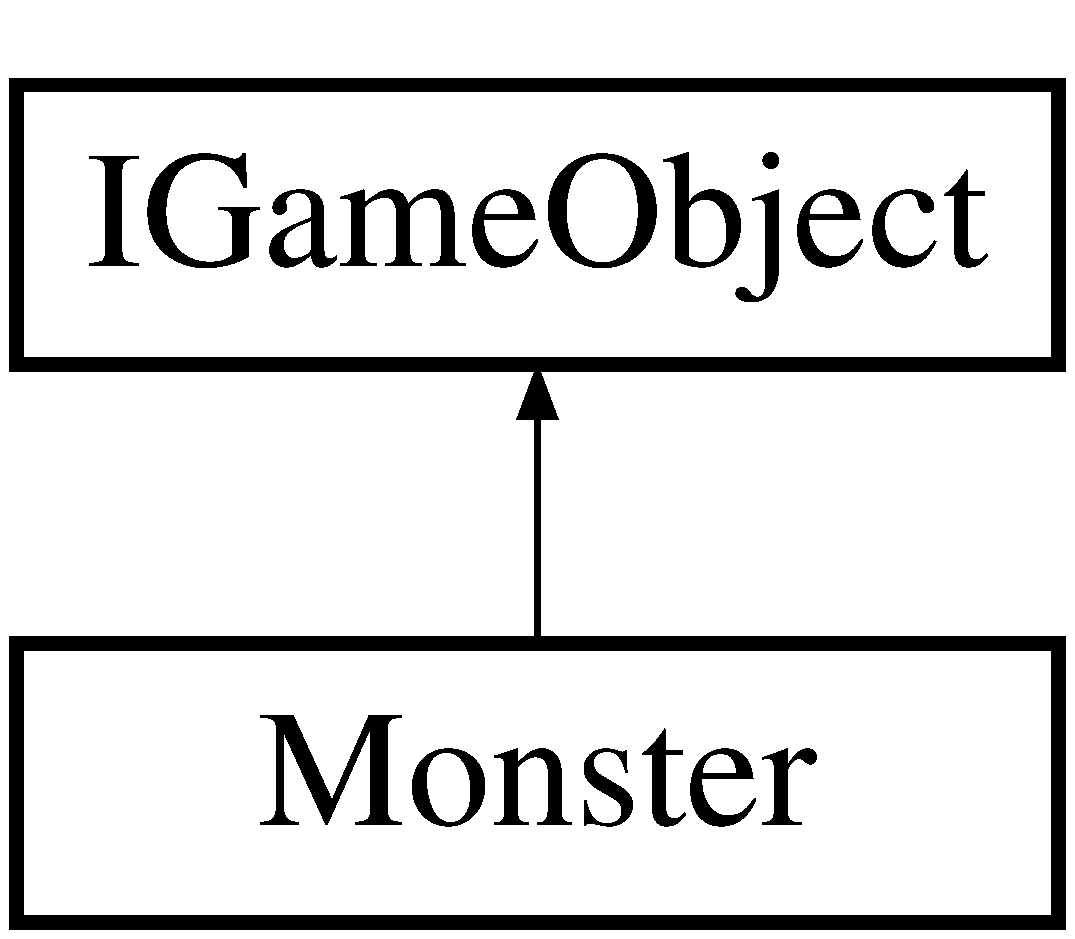
\includegraphics[height=2.000000cm]{class_monster}
\end{center}
\end{figure}
\subsection*{Public Member Functions}
\begin{DoxyCompactItemize}
\item 
virtual void \hyperlink{class_monster_ab8dc2e4d443d23c46a705aa9bc66d3dd}{Draw} () override
\begin{DoxyCompactList}\small\item\em Abstract draw method \end{DoxyCompactList}\item 
virtual void \hyperlink{class_monster_ae3cfc1c225b800d11d7f9ae864687268}{Update} (float delta\+Time) override
\begin{DoxyCompactList}\small\item\em Abstract update method \end{DoxyCompactList}\item 
virtual void \hyperlink{class_monster_a6e4cf2a4533245f65215243ef659b858}{On\+Collision} (\hyperlink{class_i_game_object}{I\+Game\+Object} $\ast$collided\+Object) override
\begin{DoxyCompactList}\small\item\em Abstract on\+Collision method \end{DoxyCompactList}\end{DoxyCompactItemize}
\subsection*{Additional Inherited Members}


\subsection{Member Function Documentation}
\hypertarget{class_monster_ab8dc2e4d443d23c46a705aa9bc66d3dd}{\index{Monster@{Monster}!Draw@{Draw}}
\index{Draw@{Draw}!Monster@{Monster}}
\subsubsection[{Draw}]{\setlength{\rightskip}{0pt plus 5cm}void Monster\+::\+Draw (
\begin{DoxyParamCaption}
{}
\end{DoxyParamCaption}
)\hspace{0.3cm}{\ttfamily [override]}, {\ttfamily [virtual]}}}\label{class_monster_ab8dc2e4d443d23c46a705aa9bc66d3dd}


Abstract draw method 

Joris, 21-\/10-\/2014. 

Implements \hyperlink{class_i_game_object_aabf746343989a0a29543a3d6db48b6a4}{I\+Game\+Object}.

\hypertarget{class_monster_a6e4cf2a4533245f65215243ef659b858}{\index{Monster@{Monster}!On\+Collision@{On\+Collision}}
\index{On\+Collision@{On\+Collision}!Monster@{Monster}}
\subsubsection[{On\+Collision}]{\setlength{\rightskip}{0pt plus 5cm}void Monster\+::\+On\+Collision (
\begin{DoxyParamCaption}
\item[{{\bf I\+Game\+Object} $\ast$}]{collided\+Object}
\end{DoxyParamCaption}
)\hspace{0.3cm}{\ttfamily [override]}, {\ttfamily [virtual]}}}\label{class_monster_a6e4cf2a4533245f65215243ef659b858}


Abstract on\+Collision method 

Joris, 21-\/10-\/2014. 


\begin{DoxyParams}{Parameters}
{\em collided\+Object} & \mbox{[}in,out\mbox{]} If non-\/null, the collided object. \\
\hline
\end{DoxyParams}


Implements \hyperlink{class_i_game_object_a31702eed0f78cff5e5d49717751bd39d}{I\+Game\+Object}.

\hypertarget{class_monster_ae3cfc1c225b800d11d7f9ae864687268}{\index{Monster@{Monster}!Update@{Update}}
\index{Update@{Update}!Monster@{Monster}}
\subsubsection[{Update}]{\setlength{\rightskip}{0pt plus 5cm}void Monster\+::\+Update (
\begin{DoxyParamCaption}
\item[{float}]{delta\+Time}
\end{DoxyParamCaption}
)\hspace{0.3cm}{\ttfamily [override]}, {\ttfamily [virtual]}}}\label{class_monster_ae3cfc1c225b800d11d7f9ae864687268}


Abstract update method 

Joris, 21-\/10-\/2014. 


\begin{DoxyParams}{Parameters}
{\em delta\+Time} & The delta time. \\
\hline
\end{DoxyParams}


Implements \hyperlink{class_i_game_object_a4959cd2f80334cfa1a97255082e984cc}{I\+Game\+Object}.



The documentation for this class was generated from the following files\+:\begin{DoxyCompactItemize}
\item 
Monster.\+h\item 
Monster.\+cpp\end{DoxyCompactItemize}

%--- End generated contents ---

% Index
\newpage
\phantomsection
\addcontentsline{toc}{chapter}{Index}
\printindex

\end{document}
